\chapter{Introduction to Ada}

In this chapter, the programming language called \emph{Ada} is introduced. We will use Ada in this subject for two reasons. First, due to its features, it is heavily used in high integrity domains, especially safety-critical systems. Second, later in the course, we will look at a language called SPARK, which is a safe programming subset of Ada, and has tool support for high integrity systems.

\section{The history of Ada}

Ada is a structured, imperative programming language with static typing, object-orientation, and concurrency built in. It was designed by a company called CII Honeywell Bull, who were contracted by the United States Department of Defence (DoD) in 1977 to provide a new language to replace the \emph{hundreds} of programming languages they were using at the time. The DoD were concerned that many of the languages were specific to particular hardware, and thus not reusable, and were becoming obsolete. Further, many of the languages did \emph{safe}, \emph{modular} programming, which had emerged as the best way to handle large-scale, complex software systems.

At the time, four contractors were asked to provide proposals for a new language, having been given a set of criteria. The  CII Honeywell Bull group's proposal was chosen as the successful proposal, and the Ada language was then designed.

Initially intended to be for embedded and real-time systems, Ada has become highly used in high integrity systems in general, especially in the safety-critical domain. Further, it was used as a general purpose programming language in the 1980s, however, due to its property of being designed to be read rather than written, many people do not consider it suitable for the more ``enterprise-y'' applications, where time-to-market is considered more important than software integrity.

The language is named after \emph{Augusta Ada King, Countess of Lovelace} (more generally known as \emph{Ada Lovelace}, who is credited as being the first even computer programmer. In 1843, when translating notes a seminar by Charles Babbage on his analytical engine (the first programmable machine) from French to English, Ada Lovelace included an addendum showing how an algorithm for calculating Bernoulli numbers using the analytical engine, which is considered the first program ever written. However, there is significant controversy as to her actual intellectual input into the algorithm, but much of this is inconsistent with Babbage's own recollection.


\section{Ada for programming ``in the large''}
   
A major criteria given by the DoD for a new programming language is that it must provide strong support for good software engineering 
  practices that scale well to very large software systems (~\(\rm
  10^6\) lines of code, and large development teams).

There are several aspects of Ada that contribute to this:

 \begin{itemize}

    \item A strong, static and safe type system. In particular, all type errors can be detected automatically at compile time.

  \item Modularity. Ada modules (called ``packages'') can be compiled separately from all other packages. Interfaces can also be compiled without the need for an implementation, meaning that some design errors can be detected before implementation begins.

  \item Information hiding. In providing interfaces/packages, Ada separates interfaces from implementation, and provides fine-grained control over visibility.

  \item Readability. This is an important aspect. Ada favours the \emph{reader} of the program over the \emph{writer}.  That is, the aim is to make Ada programs easier to read (compared to other languages), possibly at the expense of making them slightly harder to write. This is because a program is written once but read many times during maintenance.

  \item Portability. Ada does not include any platform-specific operators or data types, and can thus be compiled on many platforms.
  
  \item Standardisation. Ada is an ANSI and ISO standard.

  \end{itemize}

It is these properties, plus others, that makes Ada a great fit for high integrity systems, and is why it is still used in so many high integrity domains today. The language itself continues to evolve, and a new ISO/IEC standard for Ada was published in December 2012.

\section{Hello World}

A great way to introduce a programming language to people with programming experience is to start programs. So, let's start with a very traditional program to introduce Ada:


\lstinputlisting[caption={\textbf{hello\_world.adb}}]{\rootdir/ada/code/hello_world.adb}

Note the following about this program:

\begin{itemize}

  \item The {\bf with} statement adds the {\em Ada.Text\_IO} package
    to the program. This is basically a library import, similar to the ``import'' functionality in Java, or the \texttt{\#include} keyword in C.

  \item Block structure is given by {\bf begin}\ldots{\bf end} pairs. Thus, a procedure begins and ends with these keywords.

  \item An Ada main procedure does not need to be called ``main'', as in some other languages. Any  simple name is fine so we have used  {\em Hello\_World}.

  \item The name-space is not flat. Therefore, to access the functions declared in the \emph{Ada.Text\_IO} package, we need to prefix them with the package name.

\end{itemize}

\subsubsection*{Package renaming}

To avoid having to prefix functions with this long name each time, we can use \emph{renaming}:

\lstinputlisting[caption={\textbf{hello\_world\_renaming.adb}}]{\rootdir/ada/code/hello_world_renaming.adb}


\subsubsection*{Compiling Hello World}
  
Ada programs are divided into {\em compilation units}. An Ada \emph{specification} (or interface) is usually given the extension
      \texttt{.ads} (\textbf{AD}a \textbf{S}pecification) and the body of the program is given the extension
      \texttt{.adb} (\textbf{AD}a \textbf{B}ody).

The file name must be the same as the compilation unit name and each compilation unit must hold the name of the procedure to be compiled\footnote{Although some Ada compilers are forgiving and just produce a warning in this case}. For example, the hello world program must be placed in the file \texttt{hello\_world.adb}.

All compilation units must be compiled, bound and linked.


The notes for this subject will use the GNAT Ada compiler, which is downloadable from \url{http://libre.adacore.com/download/} for Linux and Windows (native, JVM, and .NET)... and Mindstorm!  The notes and workshops assume GNAT on Linux. Students are free to use the Windows compiler, but note that the staff cannot give much useful support on using these tools on Windows.

The GNAT Ada compiler can be used on the command line. To compile the hello world program, use the following commands:

  \begin{enumerate}
  \item \texttt{gcc -c hello\_world.adb} generates the files \texttt{hello\_world.ali} -- the
    object code -- and \texttt{hello\_world.o} -- static analysis
    information.

  \item \texttt{gnatbind hello\_world} uses \texttt{hello\_world.ali} to bind the files.

  \item \texttt{gnatlink hello\_world} uses \texttt{hello\_world.ali} to link the files.

  \end{enumerate}

Alternatively, and more conveniently, use the following:

   \begin{enumerate}
  \item \texttt{gnatmake hello\_world.adb} is a single command that performs all
    three of the above steps.
  \end{enumerate}


The result is an executable program called \texttt{hello\_world}.

You can use the command \texttt{gnatclean -c hello\_world} to delete any compiler-generated files.


\section{Specifications and program bodies}

Ada programs consist of \emph{packages}, \emph{procedures}, and \emph{functions}. Packages are synonymous with \emph{modules}, functions are defined as in other languages, and procedures are functions with no return value. More on procedures and functions later.

\emph{Specifications} show the types, functions, procedures and tasks that are publicly available for an Ada program.

As an example, we can make a simple \texttt{Greetings} package with the interface below, defined in the file \texttt{greetings.ads}:

\lstinputlisting[caption={\textbf{greetings.ads}}]{\rootdir/ada/code/greetings.ads}


This declares two procedures, \texttt{Hello} and \texttt{Goodbye}, but does not define their implementation. The package \emph{body} defines the implementation, possibly including hidden data types (we'll see an example of this later), defined in the file \texttt{greetings.adb}:

\lstinputlisting[caption={\textbf{greetings.adb}}]{\rootdir/ada/code/greetings.adb}

The names, parameter types, and return types must match between the specification and the body.

Because the two procedures are contained in a package, neither of them are directly executable. Instead, they must be executed from another procedure. Below is a code listing that calls the two procedures in succession:

\lstinputlisting[aboveskip=0ex,caption={\textbf{greetings\_main.adb}}]{\rootdir/ada/code/greetings_main.adb}

Note in this example a new keyword: \texttt{use}.  The statement \texttt{use Ada.Text\_IO} makes all of the public entities accessible without qualification in the body of the package, meaning that we no longer need to prefix \texttt{Put\_Line} with the package name. However, use this with caution: two packages can have the public entities with the same name, so importing both results in an ambiguity.

\begin{exercise}
Create two packages that contain a procedure of the same name. Import both of these using the \texttt{with} and \texttt{use} keywords, into a new program that simply calls the ambiguously declared procedure. Try to compile and run this program to see what happens.
\end{exercise}


Following the one-unit-per-file rule the program must be placed in
three separate files:

\begin{enumerate}

\item \texttt{greetings.ads}: contains the specification of the package.

\item \texttt{greetings.adb}:  contains the implementation of the package.

\item \texttt{greetings\_main.adb}: contains the main program that makes use of the \texttt{Greetings} package.

\end{enumerate}

To compile this program, we can compile the package and the program, and then bind them, as follows:

\begin{enumerate}
 \item \texttt{gcc -c gmain.adb}
 \item \texttt{gcc -c greetings.adb}
 \item \texttt{gnatbind greetings\_main}
 \item \texttt{gnatlink greetings\_main}
\end{enumerate}

Alternatively, issue the single command:

 \begin{enumerate}
 \item \texttt{gnatmake greetings\_main}
\end{enumerate}

The \texttt{gnatmake} command will locate and compile any packages used in the main program, provided that it can find them on the path. To avoid having to set up paths, we'll only deal with programs in a single directory.

\section{Comments}

Comments can be added to programs using the prefix \texttt{--}:

\begin{lstlisting}[caption={Comments}]
-- this part ignored
Put_Line("Hello, world!"); -- this part too!
\end{lstlisting}


\section{Types}

The Ada type system is a major part of its success. It is designed for programmers to create abstractions that model real world objects. As such, the type system is not based on a collection of pre-defined types, but instead, allows designers to create new types.

Of particular note in the type system are the following properties:

\begin{itemize}
    
  \item \emph{Strong typing:} types are incompatible with one another.

  \item \emph{Static typing:} type checked while compiling.

  \item \emph{Abstraction:} types represent the real world data or the problem at hand and computer representations of the data.

  \item \emph{Name equivalence:} not structural equivalence as used in most other languages. Two types are compatible if and only if they have the same name; not if they just happen to have the same size or bit representation.

\end{itemize}



\subsection{The predefined Ada type system}

Despite this, there are still a handful of predefined types in Ada. Predefined types are used as interfaces between different packages or libraries. The predefined library uses these types too.

The following predefined types are declared in the \emph{standard package}:

\begin{itemize}

    \item \textbf{Integer:} The standard integer type but must cover at least
    integers in the range \(\rm -2^{15} + 1\ldots 2^{15} -1\).

    \item \textbf{Float:} The type of floating point numbers with mantissa and
      exponent but the implementation does not follow the IEEE
      standard.

    \item \textbf{Duration:} A fixed point type used for timing and
      representing a period of time in seconds.


    \item \textbf{Character:} A special form of \emph{enumeration} type. There
      are three predefined kinds of character types: 8-bit characters,
      16-bit characters, and 32-bit characters.

    \item \textbf{String:} Three indefinite array types, of 8-bit characters,
      16-bit characters, and 32-bit characters respectively.

    \item \textbf{Boolean:} A Boolean in Ada is an enumeration of False and
      True with special semantics.
   
  \end{itemize}


  The packages \emph{System} and \emph{System.Storage\_Elements} predefine some types that are primarily useful for low-level programming and  interfacing to hardware:

  \begin{itemize}

  \item \textbf{System.Address:} An address in memory.

   \item \textbf{System.Storage\_Elements.Storage\_Offset:} An offset, which can be
    added to an address, to obtain a new address.  You can also
    subtract one address from another to get the offset between
    them. Together, {\sf Address} and {\sf Storage\_Offset} and
    their operators provide address arithmetic.


  \item \textbf{System.Storage\_Elements.Storage\_Count:} A subtype of {\sf
      Storage\_Offset} which cannot be negative, and represents the
    memory size of a data structure (similar to C's size\_t).

  \item \textbf{System.Storage\_Elements.Storage\_Element:} In most computers,
    this is a byte. Formally, it is the smallest unit of memory that
    has an address.

  \item \textbf{System.Storage\_Elements.Storage\_Array:} An array of {\sf
      Storage\_Elements} without any meaning, useful when doing raw
    memory access.

  \end{itemize}


Figure~\ref{fig:ada:type-hierarchy} shows the Ada type hierarchy. A type inherits properties from types above it in the hierarchy. 

  \begin{figure}[!h]
   \centering
    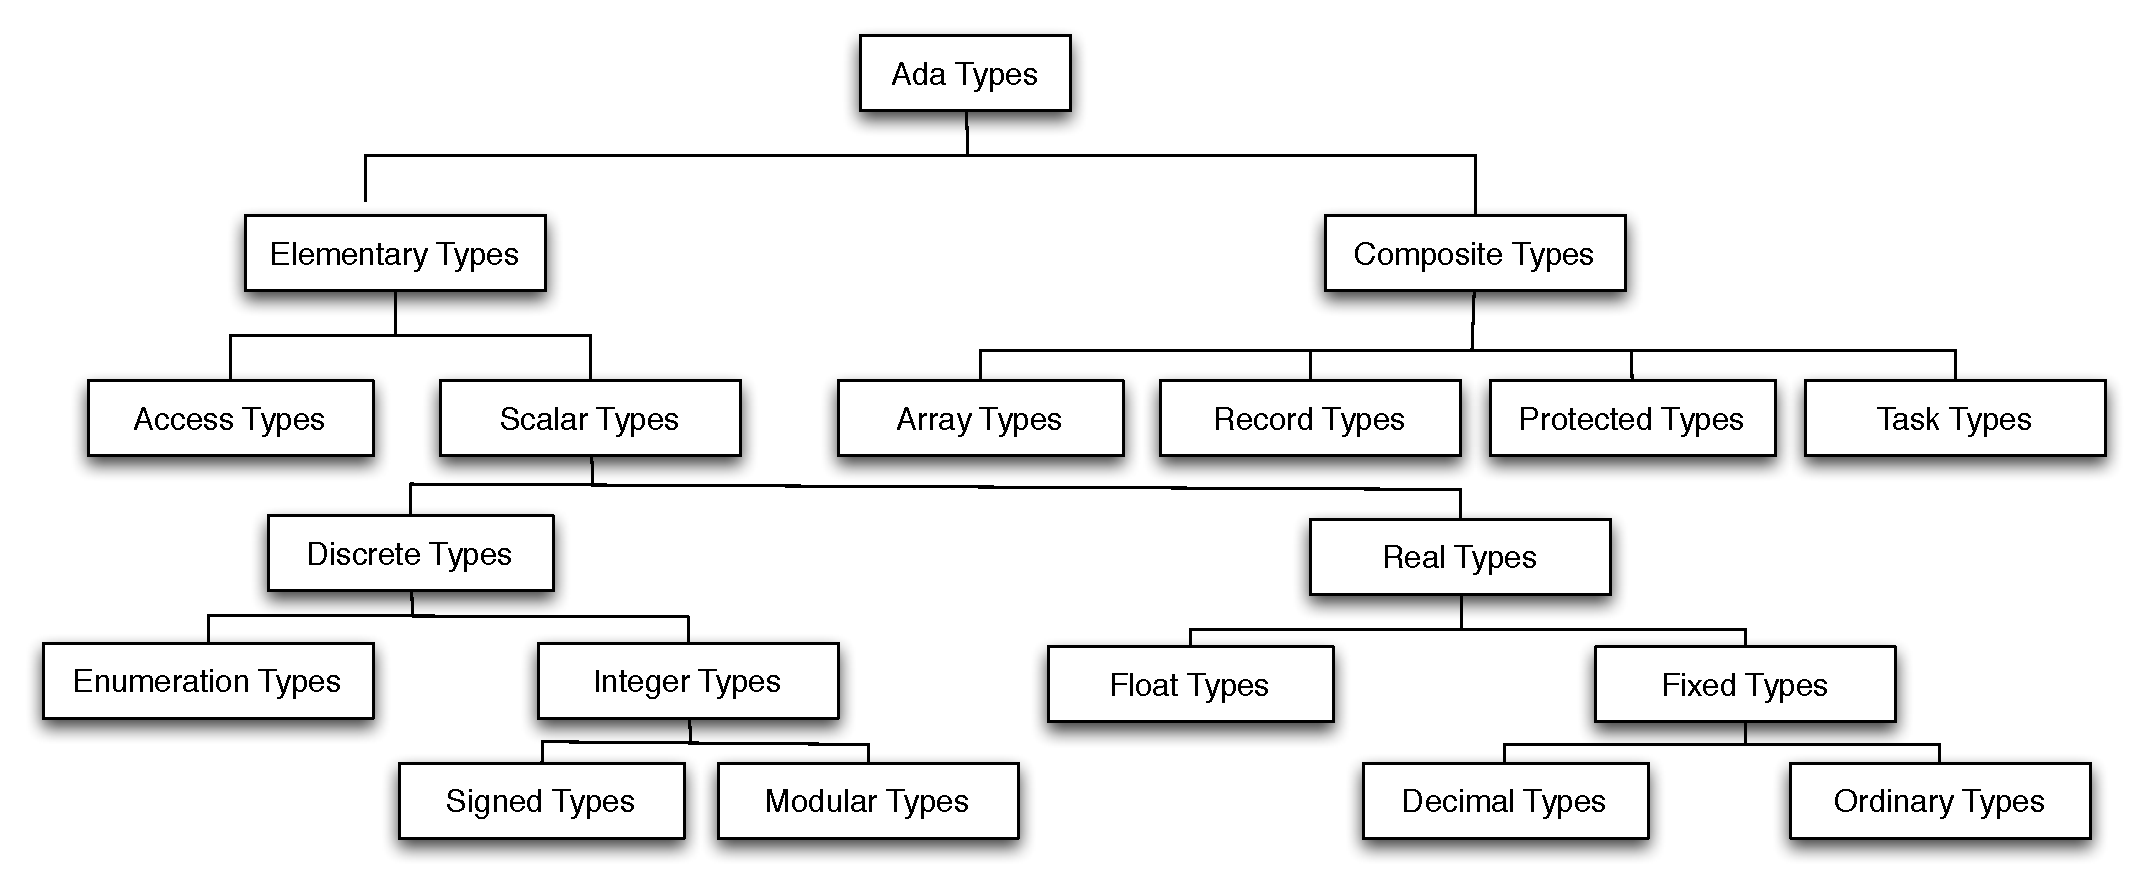
\includegraphics[scale=0.45]{\rootdir/ada//figures/AdaTypes}
   \caption{The Ada Type hierarchy.}
   \label{fig:ada:type-hierarchy}
  \end{figure}

\subsubsection{Converting to/from strings}

All scalar types (refer to Figure~\ref{fig:ada:type-hierarchy}) have two special attributes called \texttt{'Value} and \texttt{'Image}, which are used for converting to strings to values, and back. Both are functions that are called on the type, not the individual values (the Java metaphor is a static method, as opposed to an instance method).

The following code listing demonstrates how to convert a string to an integer, and back again:

  \lstinputlisting[caption={\textbf{value\_image\_attributes.adb}}]{\rootdir/ada/code/value_image_attributes.adb}

\begin{exercise}
Write a program that converts a string containing a non-number to an integer. Compile and run this program to see what happens.
\end{exercise}


 \subsection{Arrays}

Arrays in Ada are somewhat different to many other high-level programming languages -- and in fact, are more powerful as well. One key difference is in the indices of the array. In many languages, the indices of arrays are integers, starting at either 0 or 1. However, in Ada, array indices can be of any discrete type, such as characters, enumerations, etc. 

As an example, consider the following program, which declares to arrays of type \texttt{Character}, but each with a different type of index: in one case, an range of integers; and in the other, a range of characters. Elements in the array are accessed using integers for the array \texttt{Int\_Index}, but characters for the array \texttt{Ch\_Index}.

  \lstinputlisting[caption={\textbf{array\_examples.adb}}]{\rootdir/ada/code/array_examples.adb}

 Arrays have four special attributes: \texttt{'First}, \texttt{'Last}, \texttt{'Length}, and \texttt{'Range}. The first two of these do not return the first and last elements of the array, but the first and last elements of the \emph{type} of the array. Thus, in the above example, \texttt{Int\_Index'Last} will return \texttt{10}, and \texttt{Ch\_Index'First} will return the final ASCII character (null).

The \texttt{'Length} attribute returns the length of the array type (and of the array -- the entire array is allocated in Ada), while the \texttt{'Range} attribute returns the range of indices; e.g. \texttt{Int\_Index'Range} will return \texttt{5..10}.

\begin{center}
\begin{tabular}{lllll}
\toprule
\textbf{Array} &  \texttt{'First} & \texttt{'Last} & \texttt{'Length} & \texttt{'Range}\\
\midrule
 \texttt{Int\_Index} & 5 & 10 & 6 & 5..10\\
 \texttt{Ch\_Index} & $\langle$null$\rangle$ & \"y & 255 & $\langle$null$\rangle$ ..  \"y\\
\bottomrule
\end{tabular}
\end{center}

The pre-defined type \texttt{String} is a character array. However, the indices need not start at 0 or 1. Consider the following example, taken from the Ada Wikibook\footnote{See \url{http://en.wikibooks.org/wiki/Ada_Programming/Types/array}}:

\begin{lstlisting}[caption={Attributes of strings}]
Hello_World  : constant String := "Hello World!";
World        : constant String := Hello_World (7 .. 11);
Empty_String : constant String := "";
\end{lstlisting}

In this example, the attribute values are:


\begin{center}
\begin{tabular}{lllll}
\toprule
\textbf{Array} &  \texttt{'First} & \texttt{'Last} & \texttt{'Length} & \texttt{'Range}\\
\midrule
 \texttt{Hello\_World} & 1 & 12 & 12 & 1 .. 12\\
 \texttt{World} & 7 & 11 & 5 & 7 .. 11\\
 \texttt{Empty} & 1 & 0 & 0 & 1..0\\
\bottomrule
\end{tabular}
\end{center}

Thus, strings can be indexed from any range of integers, and it is not necessarily that case that \texttt{'Length = 'Last}.


  \subsection{Defining new types}
  \label{sec:ada:defining-new-types}

  A new type is introduced with the syntax:

   \textbf{\texttt{ type}}~\texttt{T}~\textbf{\texttt{is}} \ldots


   Consider the following example of defining a type for dates.

  \lstinputlisting[caption={A data type for dates}]{\rootdir/ada/code/date.ads}

  A \emph{record} is a composite type that groups one of more data type together into a single data type, similar to a \texttt{struct} in C.

  All types are incompatible with each other. Therefore, the following code snippet it illegal, because \texttt{Day\_type} and \texttt{Month\_type} are different and incompatible types, even though the  value 8 can be assigned to either:

  \begin{lstlisting}[caption={~}]
    A : Day_type := 8; 
    B : Month_type := A; -- illegal!
  \end{lstlisting}


  \section{Control Structures}

  As a structured language, the control flow of the program is structured into statements. The following control structures are the most pertinent in the Ada language.

  \begin{description}
    \item[Assignment] 

  Assignment in Ada is written as

 \texttt{X := E}

  where \texttt{X} is a variable and \texttt{E} is an expression.

   Assignment is read as ``{\em X becomes equal to E}''. 

  \item[Conditionals] {\em if-then-else} and {\em case}:

   \begin{lstlisting}[caption={A conditional}]
    if x < y then
       Put_Line ("True");
    else
       Put_Line ("False");
    end if;
  \end{lstlisting}

   \begin{lstlisting}[caption={A case statement}]
  case x is
    when 1 => Put_Line ("First");
    when 2 => Put_Line ("Second");
    when 3 => Put_Line ("Third");
    when others => Put_Line ("None!");
  end case;
  \end{lstlisting}

    \item[Unconditionals] {\em return} and {\em goto}:

    \lstinputlisting[caption={Returning a value}]{\rootdir/ada/code/use_return.adb}

    \lstinputlisting[caption={Using a goto}]{\rootdir/ada/code/use_goto.adb}


    \item[Loops] There are a number of different kinds of loops in
      Ada:

      \begin{itemize}
        \item Endless loops:

        \lstinputlisting[caption={\textbf{endless\_loop.adb}}] {\rootdir/ada/code/endless_loop.adb}


        \item While loops, which specify the termination condition at the start of the loop:

\lstinputlisting[caption={\textbf{while\_loop.adb}}] {\rootdir/ada/code/while_loop.adb}
        \item Exit loops, which specify the termination condition in the middle of the loop:

\lstinputlisting[caption={\textbf{exit\_loop.adb}}] {\rootdir/ada/code/exit_loop.adb}
        \item Until loops, which specify the termination condition at the end of the loop (which is just an exit loop with the exit condition at the end of the loop):

\lstinputlisting[caption={\textbf{until\_loop.adb}}] {\rootdir/ada/code/until_loop.adb}

        \item For loops, which allow iteration of all values in a range:

\lstinputlisting[caption={\textbf{for\_loop.adb}}] {\rootdir/ada/code/for_loop.adb}

     If the range is omitted, the loop will iterate over all possible values of the type.

       \item Array loops, which allow iteration over all elements in an array (or any other iterable types, for that matter):

\lstinputlisting[caption={\textbf{array\_loop.adb}}] {\rootdir/ada/code/array_loop.adb}



      \end{itemize}
  \end{description}




\section{Procedural Abstractions and Functional Abstractions}

The Ada language explicitly distinguishes between procedures and functions:
  
\begin{definition}
 A \emph{procedure} does not return any
  value and is considered a {\em statement}.
\end{definition}

\begin{definition}
A \emph{function} returns a value and is itself an expression.
\end{definition}

As such, functions can be used as part of larger expressions, but procedures cannot. Earlier in the hello/goodbye example (in the \texttt{Greetings} package), we saw an example of how to call a procedure (which contained no parameters). 
%An example of a function call is the \texttt{Put\_Line(..)} function call used %throughout this chapter.

For succinctness, we use the term \emph{subprogram} to include both functions and procedures.

\subsection{Parameter Modes}


When defining a procedure, each parameter of the procedure must have one of the following modes:

\begin{enumerate}

\item \texttt{in}: The formal parameter is an input parameter only, and may be read from, but cannot be written to. It is treated as a constant in the subprogram. The actual parameter value is copied into the formal parameter and is not changed by the the call. 

\item \texttt{out}: The formal parameter is an output parameter only. That is, the calling code will want to read the value of the parameter after the call is finished. The actual parameter's value before the call is irrelevant because it will get a value in the subprogram. The formal parameter may be read and written in the subprogram.

\item \texttt{in out}: The formal parameter is both an input and output parameter, and can thus be both read and written. The actual parameter may be redefined in the subprogram body. 

\item \texttt{access}: The formal parameter is an \emph{access type} (a pointer) to some variable.

\end{enumerate}

If a parameter is declared without one of these modes, then by default, its mode is \texttt{in}.

For functions, parameters must be of mode \texttt{in} or \texttt{access}.  To write a subprogram that returns more than one value, the return values must be all \texttt{out} parameters.


\subsection{Calling subprograms}

There are three syntax variations for calling subprograms:

\begin{enumerate}

 \item Calling subprograms that have no parameters -- called as just the subprogram name with no brackets.

 \item Calling via positional arguments. This is found in most high-level programming languages, in which the position of the arguments in the call must be the same as in the declared subprogram.

 \item Calling via named associations. This is where parameter variable names are explicitly specified in the calling code.

\end{enumerate}

The code listing below provides examples of all three call types:

\lstinputlisting[caption={\textbf{calling\_subprograms.adb}}] {\rootdir/ada/code/calling_subprograms.adb}

Note that the order of the arguments in the final call (using named associations) is different to the declared order.

\section{Example: Insertion sort}

Before we go any further, it is time for a complete example. The example we use is \emph{insertion sort}\footnote{Taken from Rosetta Code: \url{http://rosettacode.org/wiki/Sorting_algorithms/Insertion_sort\#Ada}} -- a well-known sorting algorithm with worst-case complexity $O(n^2)$, which works by finding the smallest remaining element in the unsorted part of the array and inserting it at the end of the sorted part of the array. This example uses many of the constructs seen already, declaring the procedure in a package. 

The package specification consists of a type declaration and a procedure declaration:

\lstinputlisting[caption={\textbf{sort.ads}}] {\rootdir/ada/code/sort.ads}

The package body implements the procedure specification:

\lstinputlisting[caption={\textbf{sort.adb}}] {\rootdir/ada/code/sort.adb}

The following serves as a small demonstrating of creating an unsorted array, sorting it, and printing the result:


\lstinputlisting[caption={\textbf{sort\_main.adb}}] {\rootdir/ada/code/sort_main.adb}

\section{Concurrency with tasks}

 The final topic that we cover in this chapter is \emph{tasks}. Tasks are the basic unit of concurrency in Ada.  As such, they are much like threads in Java -- but have several differences.

Tasks are important in Ada because they help to support real-time systems. Many (perhaps most?) safety- and mission-critical systems are real-time. That is, timing is part of the functional specification of the system, and failure to complete some function before a deadline means that the system has failed.

Tasks start executing the moment they are created. Tasks are not called, unlike functions and procedures. Tasks can communicate with other tasks:

  \begin{itemize}

  \item Tasks can pass messages -- message passing;

  \item Tasks can share variables -- shared memory communication.

  \end{itemize}

Ada programs and tasks are scheduled. Unlike programs, the effects of task scheduling are often visible. 

The example below\footnote{Taken from \url{https://en.wikibooks.org/wiki/Ada_Programming/Tasking}} shows the declaration and body of two tasks: one for ``backing up'' and one for ``cleaning the CPU''.

\lstinputlisting[caption={\textbf{housekeeping.adb}}] {\rootdir/ada/code/housekeeping.adb}

The master of the tasks is the procedure \texttt{Housekeeping}. The procedure itself does nothing except declare the tasks, which then execute automatically. The body of \texttt{Housekeeping} is empty and just waits for its child tasks to terminate.


\subsubsection*{Entry points}

Tasks communicate with each other via \emph{entry points} (or \emph{entry calls}). Tasks can have one or more entry points. Explicitly named \emph{entry points} are declared in the task declaration.


The \texttt{entry} keyword declares an entry point into a task.  Entries are declared in much the same way as procedures. They have identifiers and parameters (which can be \texttt{in}, \texttt{out}, or \texttt{in out} parameters).

An entry is executed by the called task, not the calling task. The calling task is suspended until the call completes. If the called task cannot process the entry call immediately (most commonly because it is already executing on behalf of another call), the call is placed in a FIFO queue associated with that entry.


This interaction between calling task and called task is known as a
\emph{rendezvous}. A task accepts rendezvous with any caller for a specific entry by executing an \emph{accept} statement for that entry.

The following code snipped demonstrates how entry and accept statements work:

\lstinputlisting[caption={\textbf{entry\_call.adb}},label={listing:ada:entry_call.adb}] {\rootdir/ada/code/entry_call.adb}

The above example also demonstrates several other important aspects of tasks:

\begin{enumerate}

 \item \emph{Task types}: The two tasks used are of the same \emph{task type}, \texttt{Encapsulated\_Variable\_Task\_Type}. This allows tasks to be created \emph{dynamically}, and also included into new data structures.

 \item \emph{Selective waits}: The \texttt{select} keyword is used to prevent a task being held up when it could be doing something. In the above example, the task can choose between storing or fetching an item. If there is only one pending call, that is executed. If there is more than one, \emph{any} of the tasks can be chosen, thus introducing non-determinism into the program.

 \item \emph{Termination}: The loop in the tasks above will execute indefinitely. By giving the tasks a \texttt{termination} alternative, they will terminate when: (1) they have no pending calls; (2) no other tasks that are children of the task's master have any pending calls; and (3) the task's master has completed.

\end{enumerate}

\begin{exercise}
Remove the \texttt{terminate} statement from the \texttt{Encapsulated\_Variable\_Task\_Type} task and re-run the example.
\end{exercise}

\subsubsection*{Guards}

Entries can have guards that only allow the entry to execute under specific circumstance. For example, in Listing~\ref{listing:ada:entry_call.adb}, we could add a guard to the \texttt{Store} entry restricting the input to under certain numbers:

\begin{lstlisting}[caption={~}]
     when An_Integer < 100 =>
        accept Insert (An_Integer : in Integer) do
\end{lstlisting}

A guard means that this entry point is not open, another entry point can be executed.

\section{Further reading}

An excellent introduction to Ada, which includes chapters on systems programming, real-time systems, generic types, and distributed systems, is Ben-Ari's book ``\emph{Ada for Software Engineers}'' \cite{ben2009ada}. This is available as an e-book from the University of Melbourne library, and is far more comprehensive than these notes.

A excellent online reference is the ``Ada programming'' Wikibook \cite{ada-wikibook}, which offers a substantial overview of the Ada language and many complete examples, some of which are used in this chapter.



% LocalWords:  CII DoD IEC adb pecification ody downloadable JVM Mindstorm gcc
% LocalWords:  ali gnatbind gnatlink gnatmake gnatclean aboveskip gmain pre Int
% LocalWords:  Index'Last Ch Index'First Index'Range Wikibook Unconditionals
% LocalWords:  iterable Ari's  practices IEEE indices lllll online
